\documentclass[a4paper]{ctexart}
\usepackage{ctex}
\usepackage{times}
\usepackage{setspace}
\usepackage{fancyhdr}
\usepackage{graphicx}
\usepackage{wrapfig}
\usepackage{array}
\usepackage{fontspec,xunicode,xltxtra}
\usepackage{titlesec}
\usepackage{titletoc}
\usepackage[titletoc]{appendix}
\usepackage[top=30mm,bottom=30mm,left=20mm,right=20mm]{geometry}
\usepackage{enumerate}
\usepackage{caption}
\usepackage{abstract}
\usepackage{microtype}
\usepackage{amsmath}
\usepackage{listings}
\usepackage{color}

\setmainfont{TeX Gyre Pagella}

\definecolor{codegreen}{rgb}{0,0.6,0}
\definecolor{codegray}{rgb}{0.5,0.5,0.5}
\definecolor{codepurple}{rgb}{0.58,0,0.82}
\definecolor{backcolour}{rgb}{0.95,0.95,0.92}

\captionsetup[figure]{name={图},labelsep=period,font={bf,small}}

%---------------------------------------------------------------------
%	页眉页脚设置
%---------------------------------------------------------------------
\fancypagestyle{plain}{\pagestyle{fancy}}%改变章节首页页眉
\pagestyle{fancy}
\lhead{\kaishu~单片机课程设计报告~}
\rhead{\kaishu~1030616134~尹达恒~}
\cfoot{\thepage}

%---------------------------------------------------------------------
%	目录页设置
%---------------------------------------------------------------------
\renewcommand{\contentsname}{\zihao{-3}{\centerline{目录}}}
\titlecontents{section}[2em]{\vspace{0.1\baselineskip}\songti\zihao{-4}}{\thecontentslabel\ }{}
{\hspace{.5em}\titlerule*[4pt]{$\cdot$}\contentspage}
\titlecontents{subsection}[4em]{\vspace{0.1\baselineskip}\songti\zihao{-4}}{\thecontentslabel\ }{}
{\hspace{.5em}\titlerule*[4pt]{$\cdot$}\contentspage}
\titlecontents{subsubsection}[6em]{\vspace{0.1\baselineskip}\songti\zihao{-4}}{\thecontentslabel\ }{}
{\hspace{.5em}\titlerule*[4pt]{$\cdot$}\contentspage}

%---------------------------------------------------------------------
%	章节编号设置
%--------------------------------------------------------------------
\ctexset {
	section = {
		number = \arabic{section},
		format = \zihao{4}\bfseries,
	},
	subsection = {
		number = \arabic{section}.\arabic{subsection},
		format = \zihao{-4}\bfseries,
	},
	subsubsection = {
		number = \arabic{section}.\arabic{subsection}.\arabic{subsubsection},
	}
}

\newcommand{\thskp}{\hskip 8pt}
\newcommand{\hskpthr}{\hskip 15.75pt}
\begin{document}
%---------------------------------------------------------------------
%	封面页
%---------------------------------------------------------------------
\begin{titlepage}
	\begin{center}
    
\includegraphics[width=0.9\textwidth]{figure//Njust.png}\\[64pt]
    \textbf{\fontsize{32pt}{32pt}\heiti{单\thskp 片\thskp 机\thskp 课\thskp 程\thskp 设\thskp 计\thskp 报\thskp 告}}\\[64pt]
    \textbf{\zihao{2}\songti{基于Arduino单片机的平衡车控制系统}}\\[3cm]
	\vspace{\fill}
	\setlength{\extrarowheight}{3mm}
	{\songti\zihao{3}
		\kaishu{\thskp 物联网工程\thskp}\songti{学院}\kaishu{\thskp 物联网工程\thskp}\songti{专业}\\
		\begin{tabular}{rl}
			{\makebox[4\ccwd][s]{班\qquad 级:}}& ~\kaishu 物联1601\\
			{\makebox[4\ccwd][s]{姓\qquad 名:}}& ~\kaishu 尹达恒\\ 
			{\makebox[4\ccwd][s]{学\qquad 号:}}& ~\kaishu 1030616134\\ 
			{\makebox[4\ccwd][s]{指导老师:}} & ~\kaishu 孙顺远\\ 
		\end{tabular}
	}\\[2cm]
	\vspace{\fill}
	\zihao{4}
	2018\textasciitilde 2019第一学期\\
	\today
	\end{center}
\end{titlepage}

%---------------------------------------------------------------------
%  目录页
%---------------------------------------------------------------------
\tableofcontents % 生成目录
\newpage

%---------------------------------------------------------------------
%  正文
%---------------------------------------------------------------------
\begin{spacing}{1.5}%这是段落间距
\songti\zihao{-4}
\section{设计任务}
组装一辆两轮车,并通过编程和参数调节使其在接通电源的情况下保持一定程度的直立。
\section{设计内容}
\subsection{部件及特性}
\subsubsection{框架}
小车框架一共使用了约200粒LEGO科技积木。
\subsubsection{电机}
小车电机选用LEGO EV3 45502/95658 大号伺服电机,该电机属于减速电机,且内部集成了一个绝对式编码盘用于测量电机位置。
主要特性如下\footnote{数据来源http://www.coolbricks.com/motoren}:
\begin{itemize}
	\item 额定电压:9V
	\item 空载电流:60mA
	\item 空载转速:175r/min
	\item 堵转转矩:43Ncm
	\item 堵转电流:1.8A
	\item 编码盘精度:1$^\circ$
\end{itemize}
\subsubsection{电机驱动}
小车电机驱动选用开源硬件Bricktronics Motor Driver。其主要特性如下\footnote{数据来源:https://www.wayneandlayne.com/projects/bricktronics-motor-driver/}:
\begin{itemize}
	\item 最多驱动两路LEGO EV3电机
	\item 电机驱动输入电压:9V
	\item PWM输入和编码器数据输出电压:5V
	\item 编码器数据输出方式:标志IIC通信协议
\end{itemize}
\subsubsection{传感器}
小车传感器选用MPU6050三轴加速度计电子陀螺仪。其主要特性如下:
\begin{itemize}
	\item 使用芯片:MPU6050
	\item 供电电压:3-5V
	\item 通信方式:标准IIC通信协议
	\item 芯片内置:16bit AD转换器,16位数据输出
	\item 陀螺仪测量范围:$\pm$250 500 1000 2000$^\circ$/s
	\item 加速度范围:$\pm$2 $\pm$4 $\pm$8 $\pm$16g
	\item 引脚间距:2.54mm
\end{itemize}
\subsubsection{主控制器}
小车主控制器选用Arduino uno R3单片机,主要特性如下:
\begin{itemize}
	\item 芯片:ATmega328P
	\item 工作电压:5V
	\item 输入电压(推荐):7-12V
	\item 输入电压(限值):6-20V
	\item 数字输入/输出引脚:14路(其中6路可用于PWM输出)
	\item PWM数字I/ O引脚:6 
	\item 模拟输入引脚:6
	\item 输入/输出电流:20 mA
	\item 闪存存储器:32KB,其中引导程序0.5KB
	\item SRAM:2KB
	\item EEPROM:1KB
	\item 时钟频率:16MHz
\end{itemize}
\subsubsection{无线调试模块}
小车选用一对443Wifi模块和一个TTL转USB串口模块组成无线调试模块。上位机使用山外多功能调试助手。
\subsubsection{电源}
小车选用9V集成充电电池为Arduino和电机供电,电池接口为标准9V集成电池盒。
\subsection{结构}
\subsubsection{电路结构}
传感器、马达驱动和Arduino的电路连接方式如图\ref{circ}。
\begin{figure}[htbp]
	\centering
	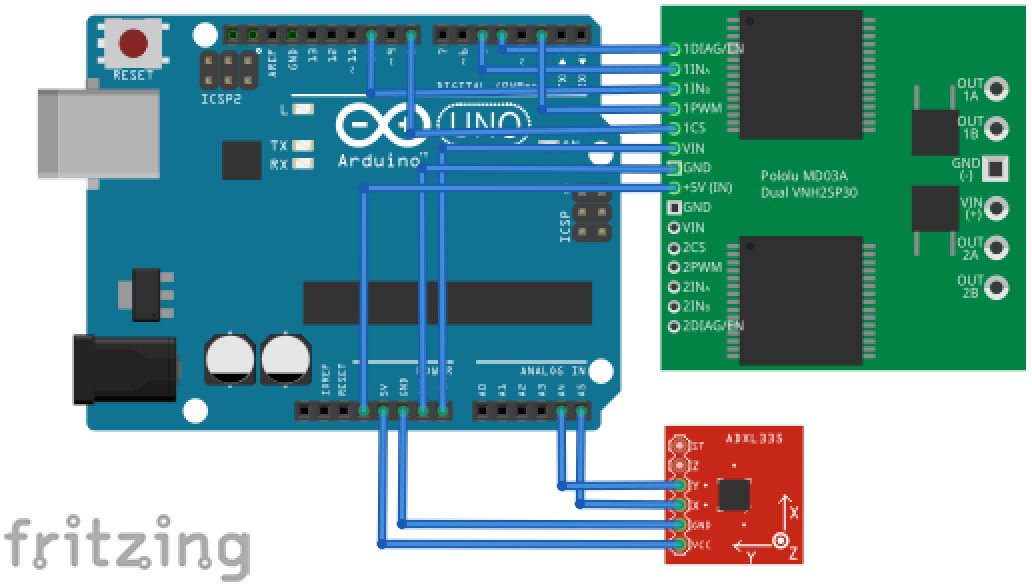
\includegraphics [width=\textwidth]{figure//circ.png}
	\caption{电路连接图}\label{circ}
\end{figure}
\subsubsection{机械结构}
\begin{enumerate}
	\item LEGO组件:考虑到小车总体框架结构简单,零件数量不多,因此不采用LDD工具进行框架设计,而直接采用“由简至繁,逐步稳固”的拼接原则,设计组装同步进行。
	\item 非LEGO组件:对于非LEGO组件的连接,这里选用M3螺母和M3*10螺丝或M3*6单通六角铜柱将非LEGO组件栓在乐高组件的十字孔上连接方式(如图\ref{link})。
	\begin{figure}[htbp]
		\begin{minipage}[t]{0.505\textwidth}
			\centering
			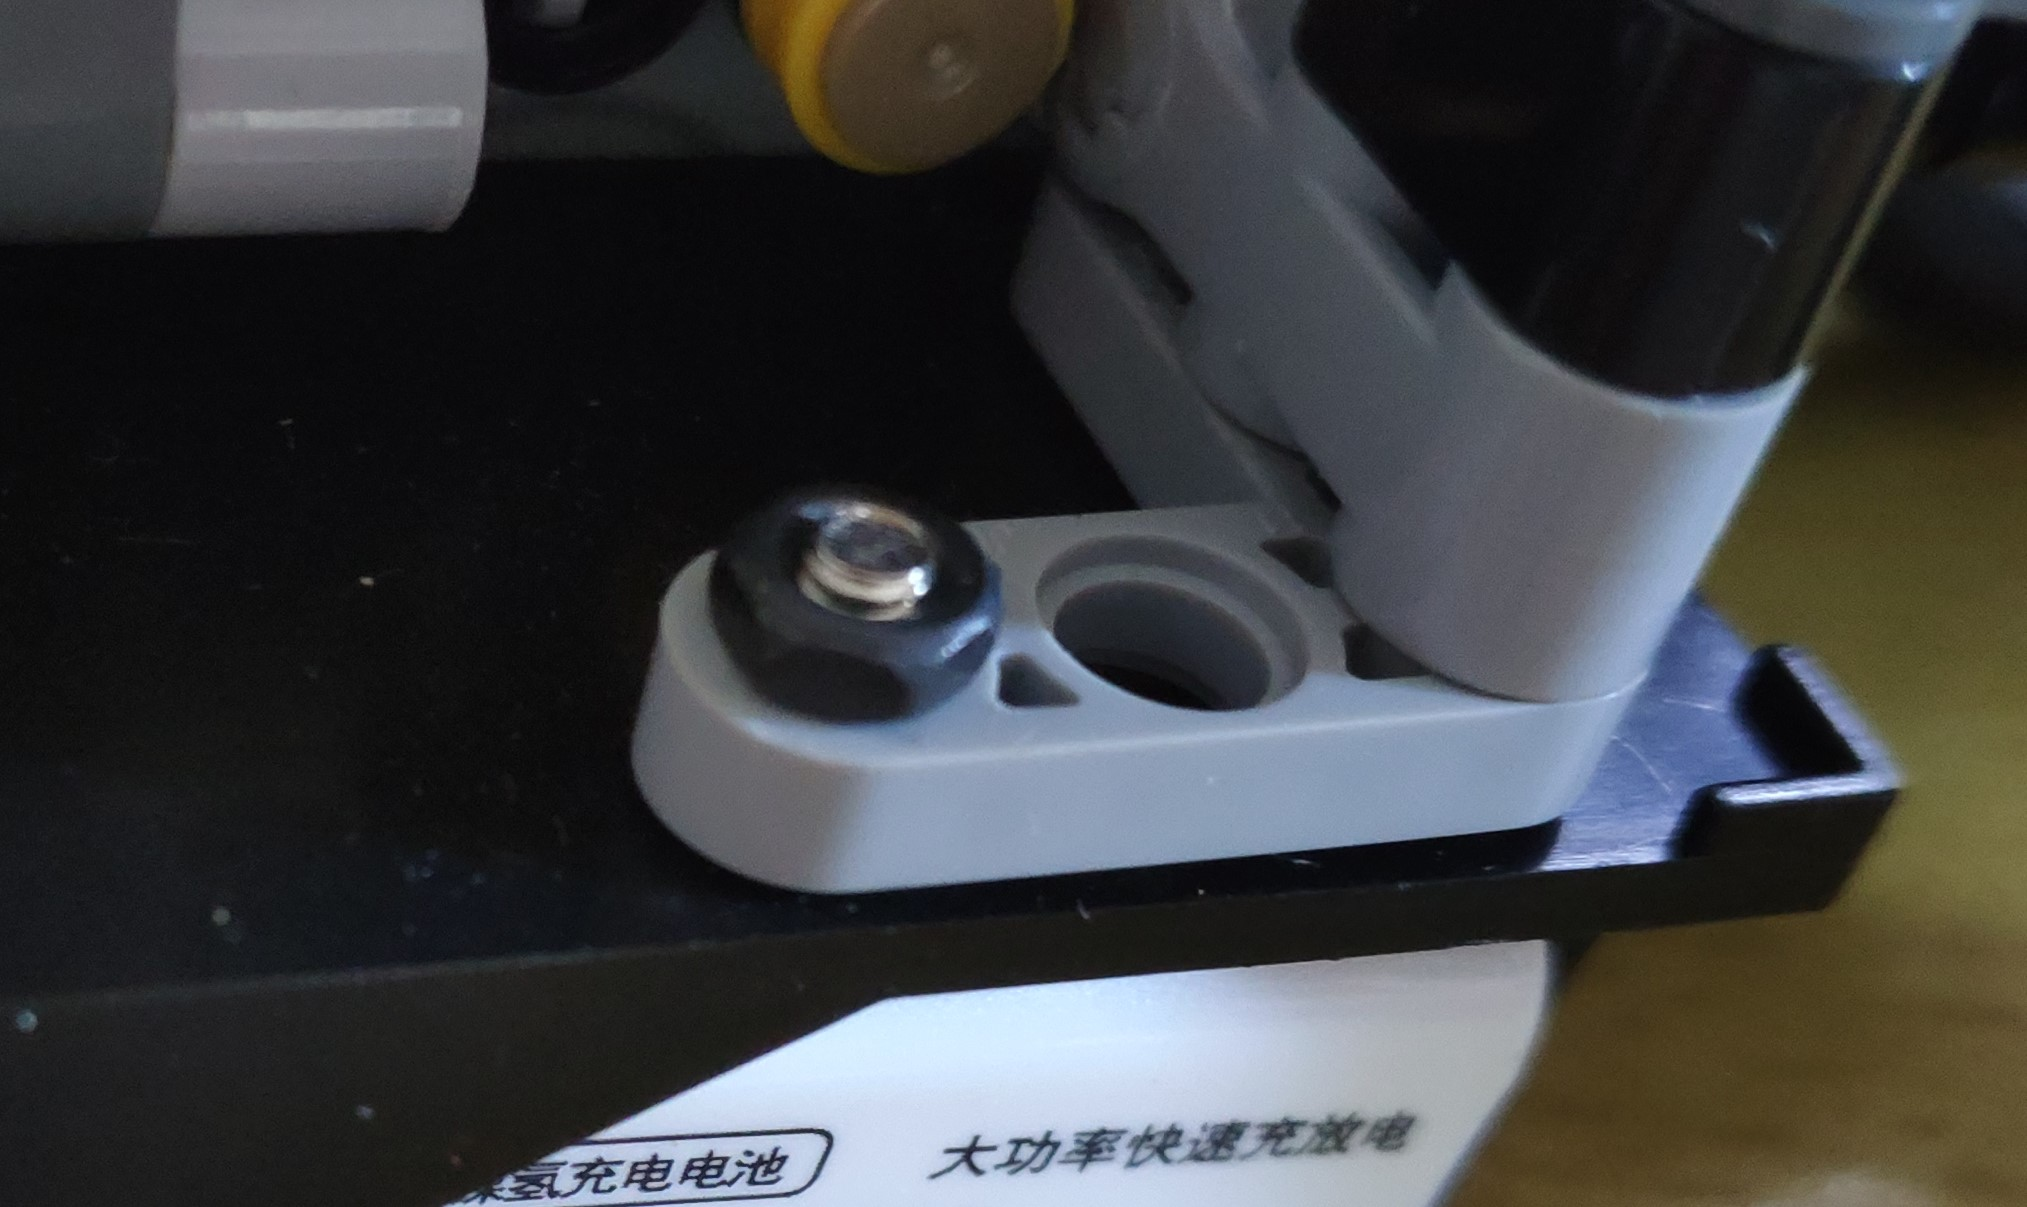
\includegraphics[width=\textwidth]{figure//L1.jpg}
			\caption*{螺栓连接}
		\end{minipage}%
		\hfill
		\begin{minipage}[t]{0.495\textwidth}
			\centering
			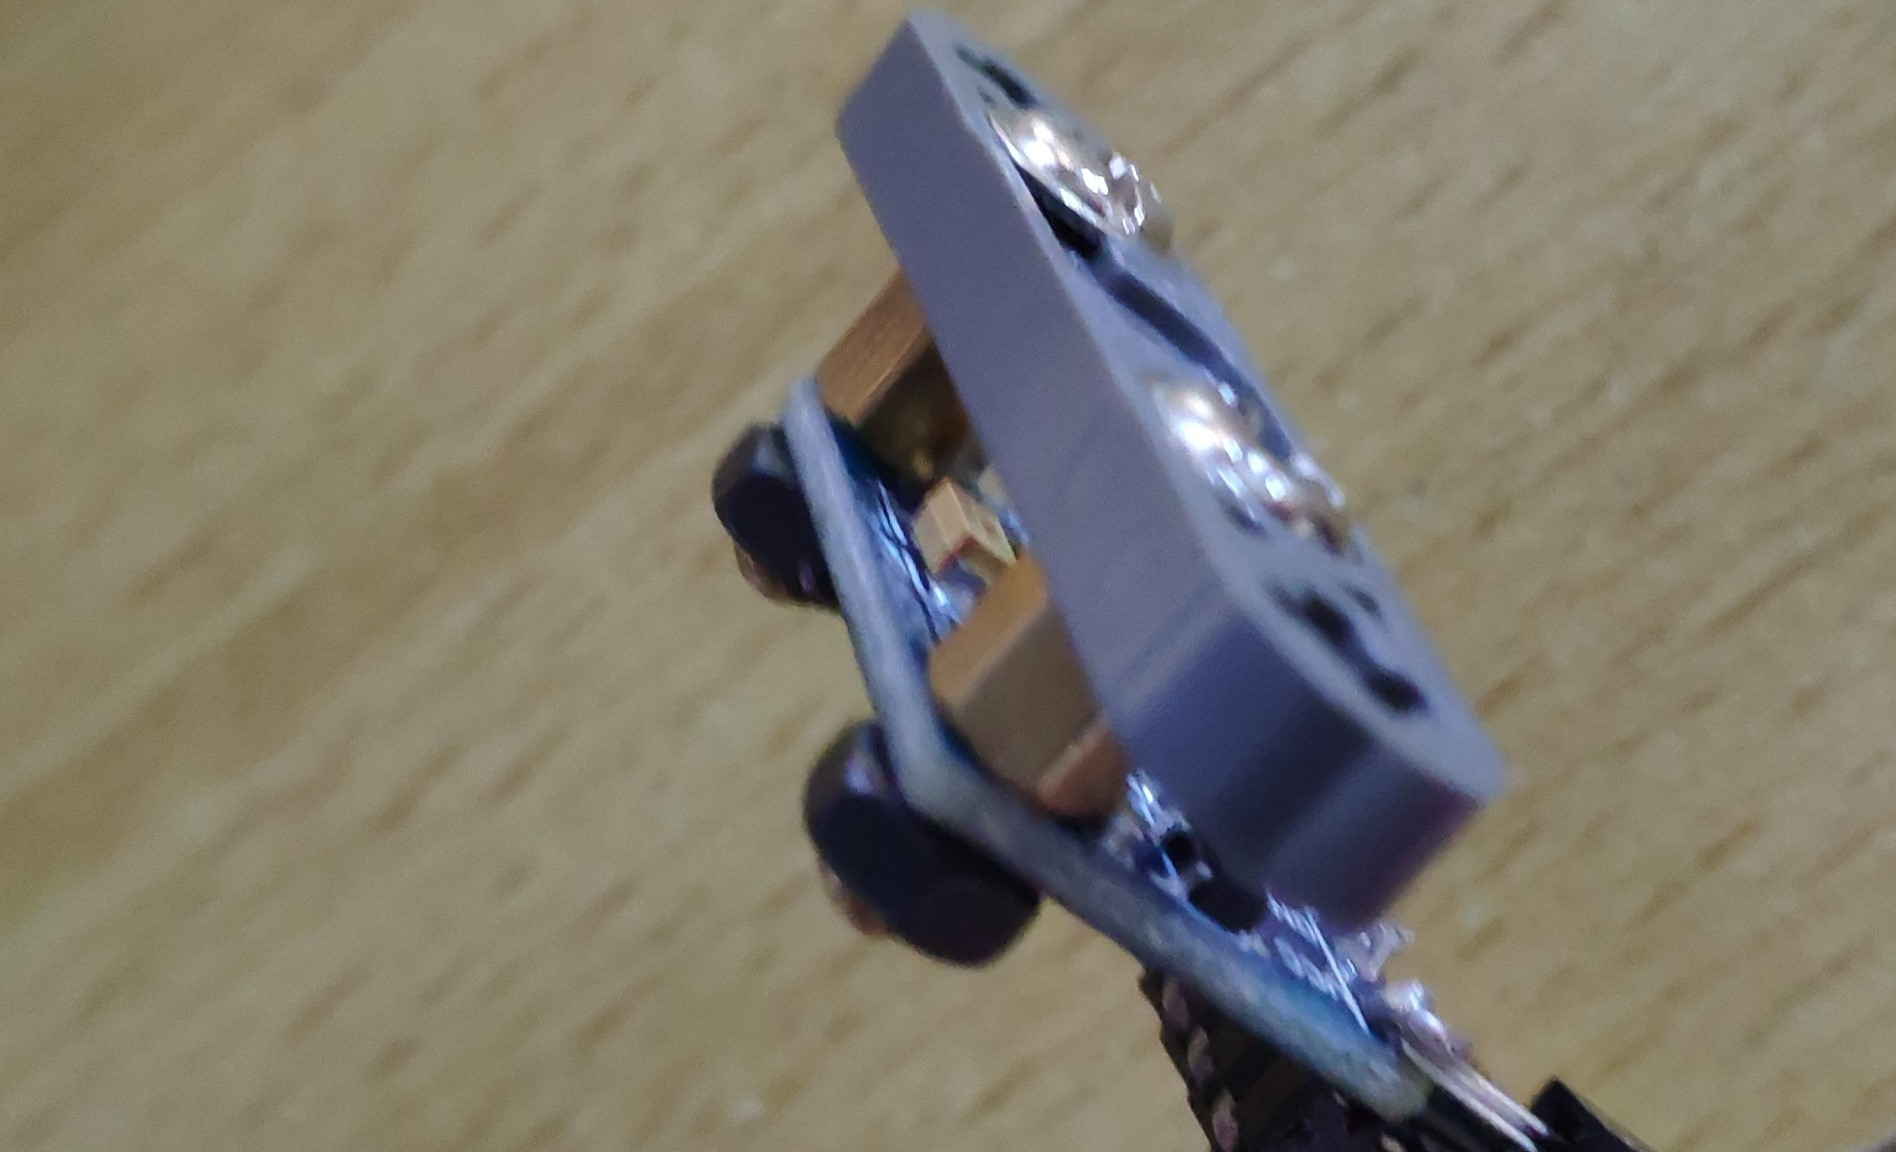
\includegraphics[width=\textwidth]{figure//L2.jpg}
			\caption*{铜柱连接}
		\end{minipage}
		\caption{非LEGO组件的连接方式}\label{link}
	\end{figure}
\end{enumerate}
小车最终的实物结构如图\ref{frame}
\begin{figure}[htbp]
\begin{minipage}[t]{0.476\textwidth}
	\centering
	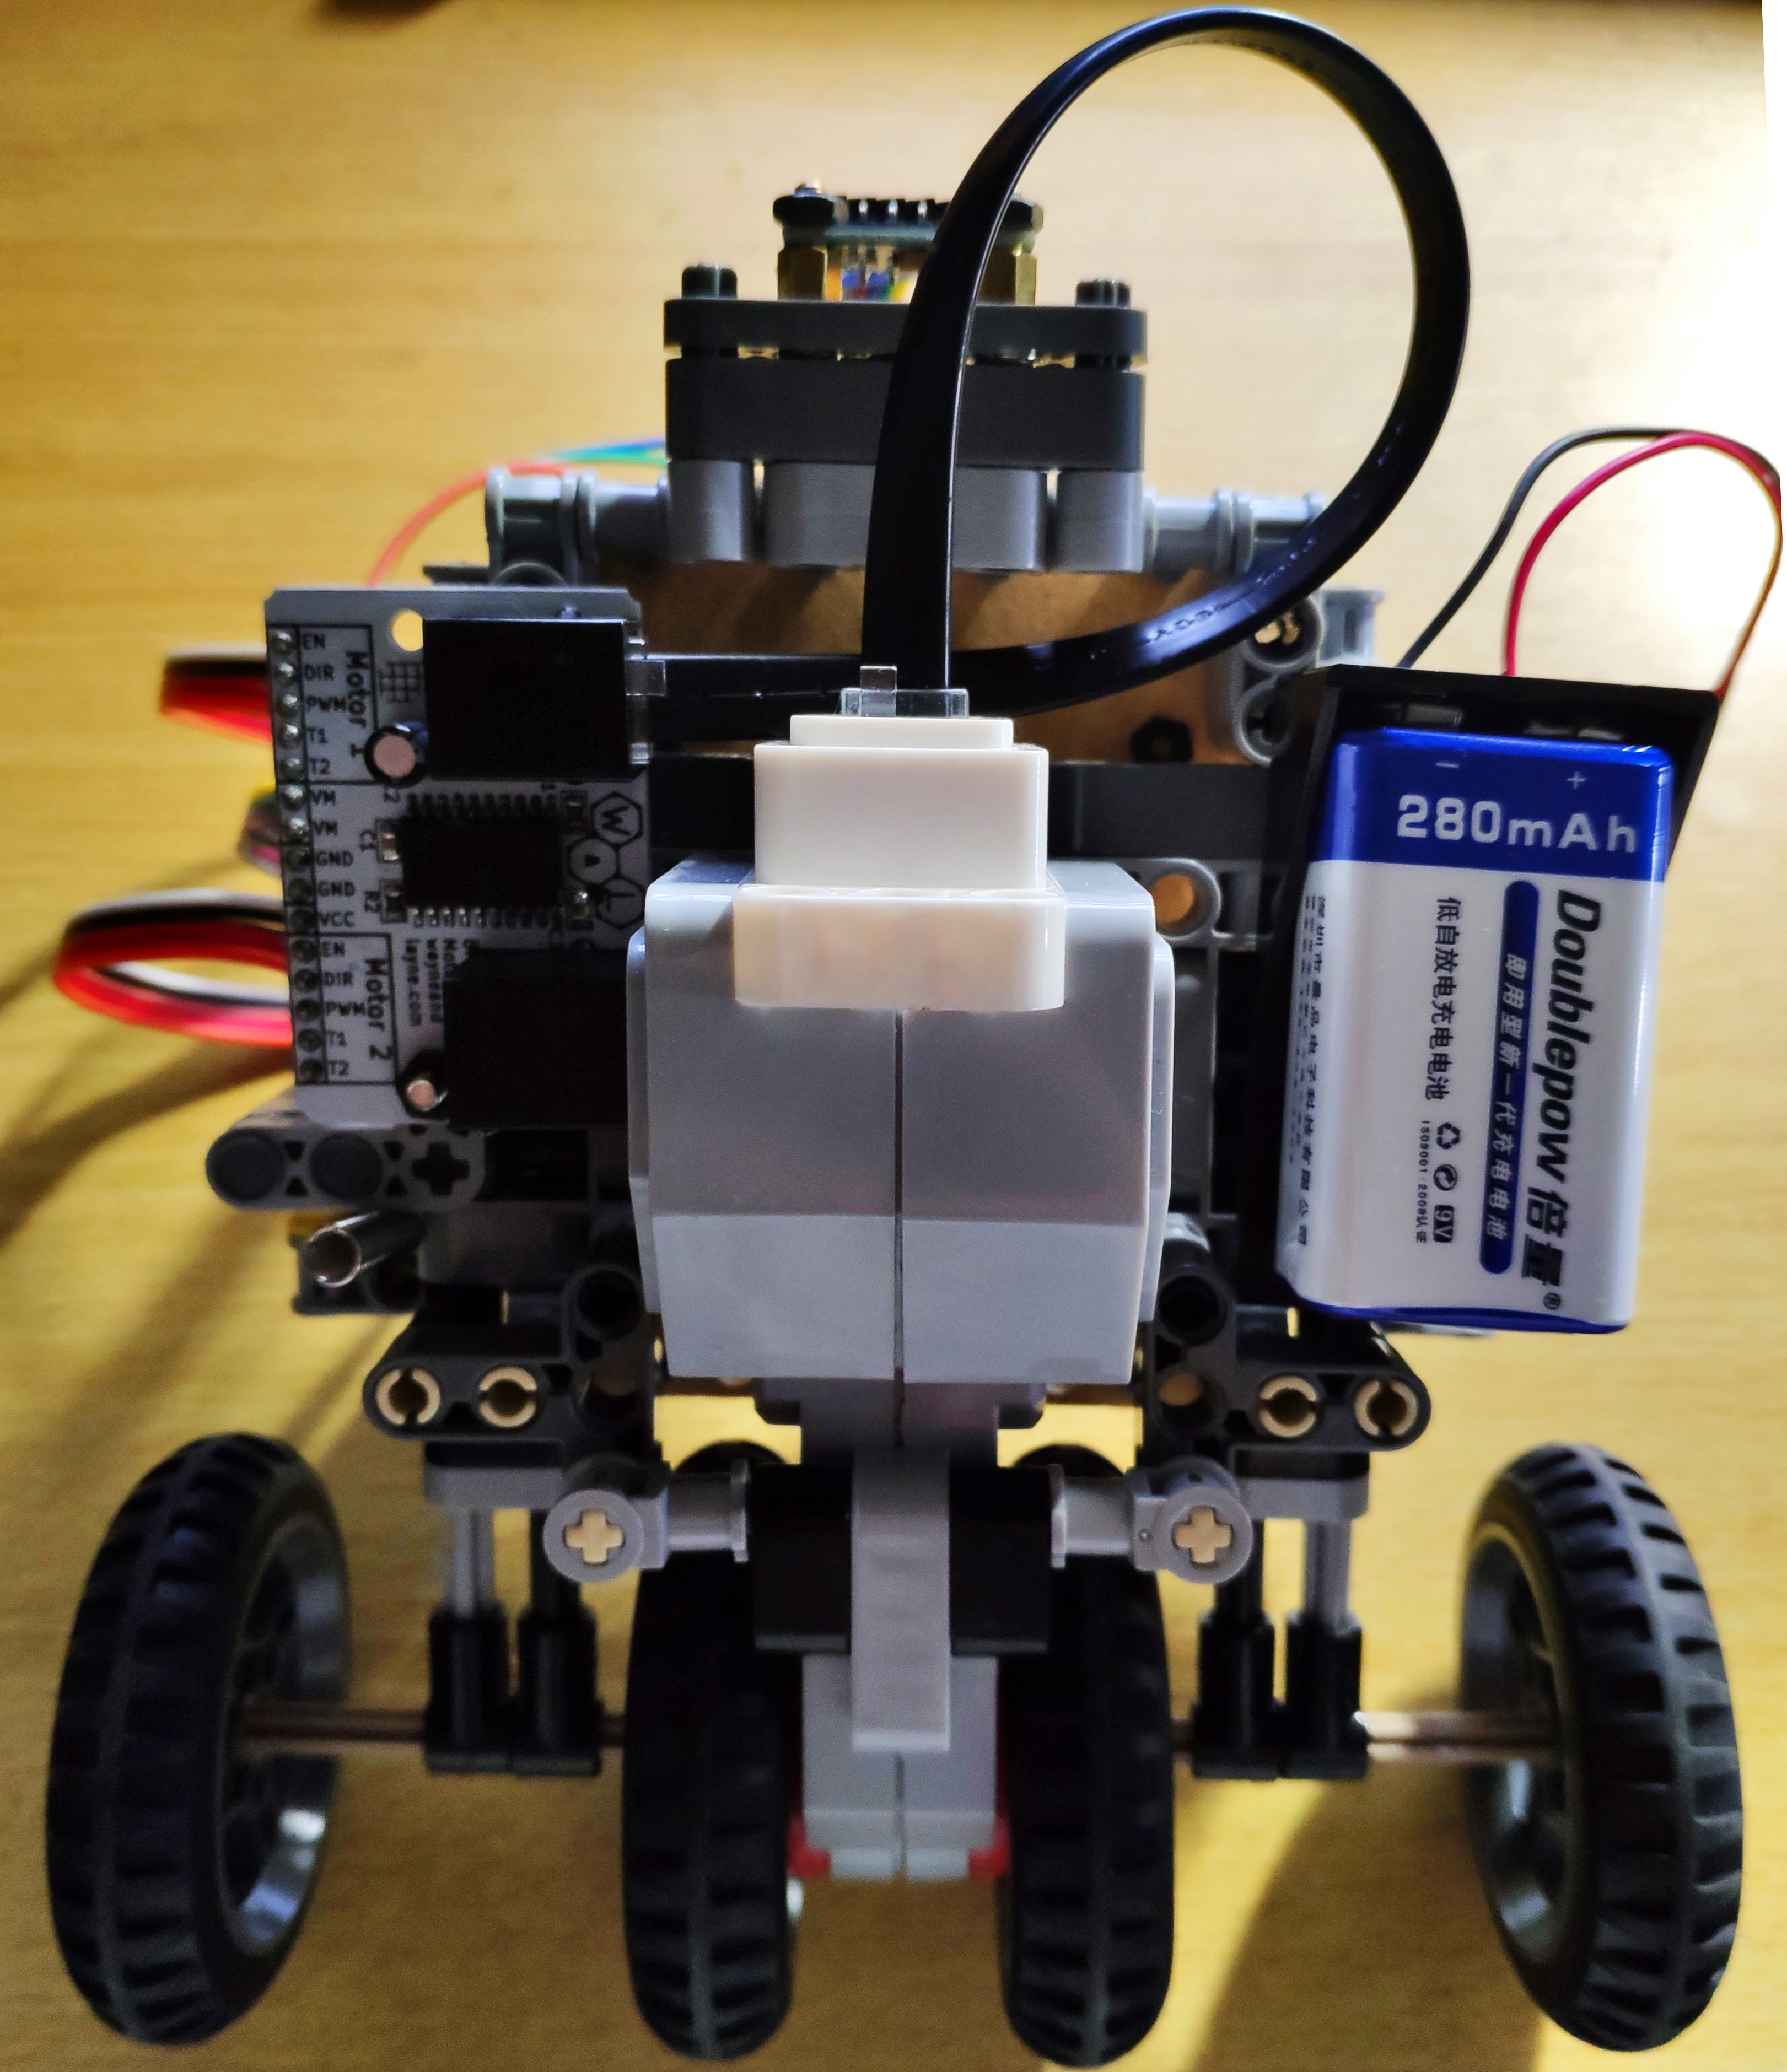
\includegraphics[width=\textwidth]{figure//F1.jpg}
\end{minipage}%
\hfill
\begin{minipage}[t]{0.524\textwidth}
	\centering
	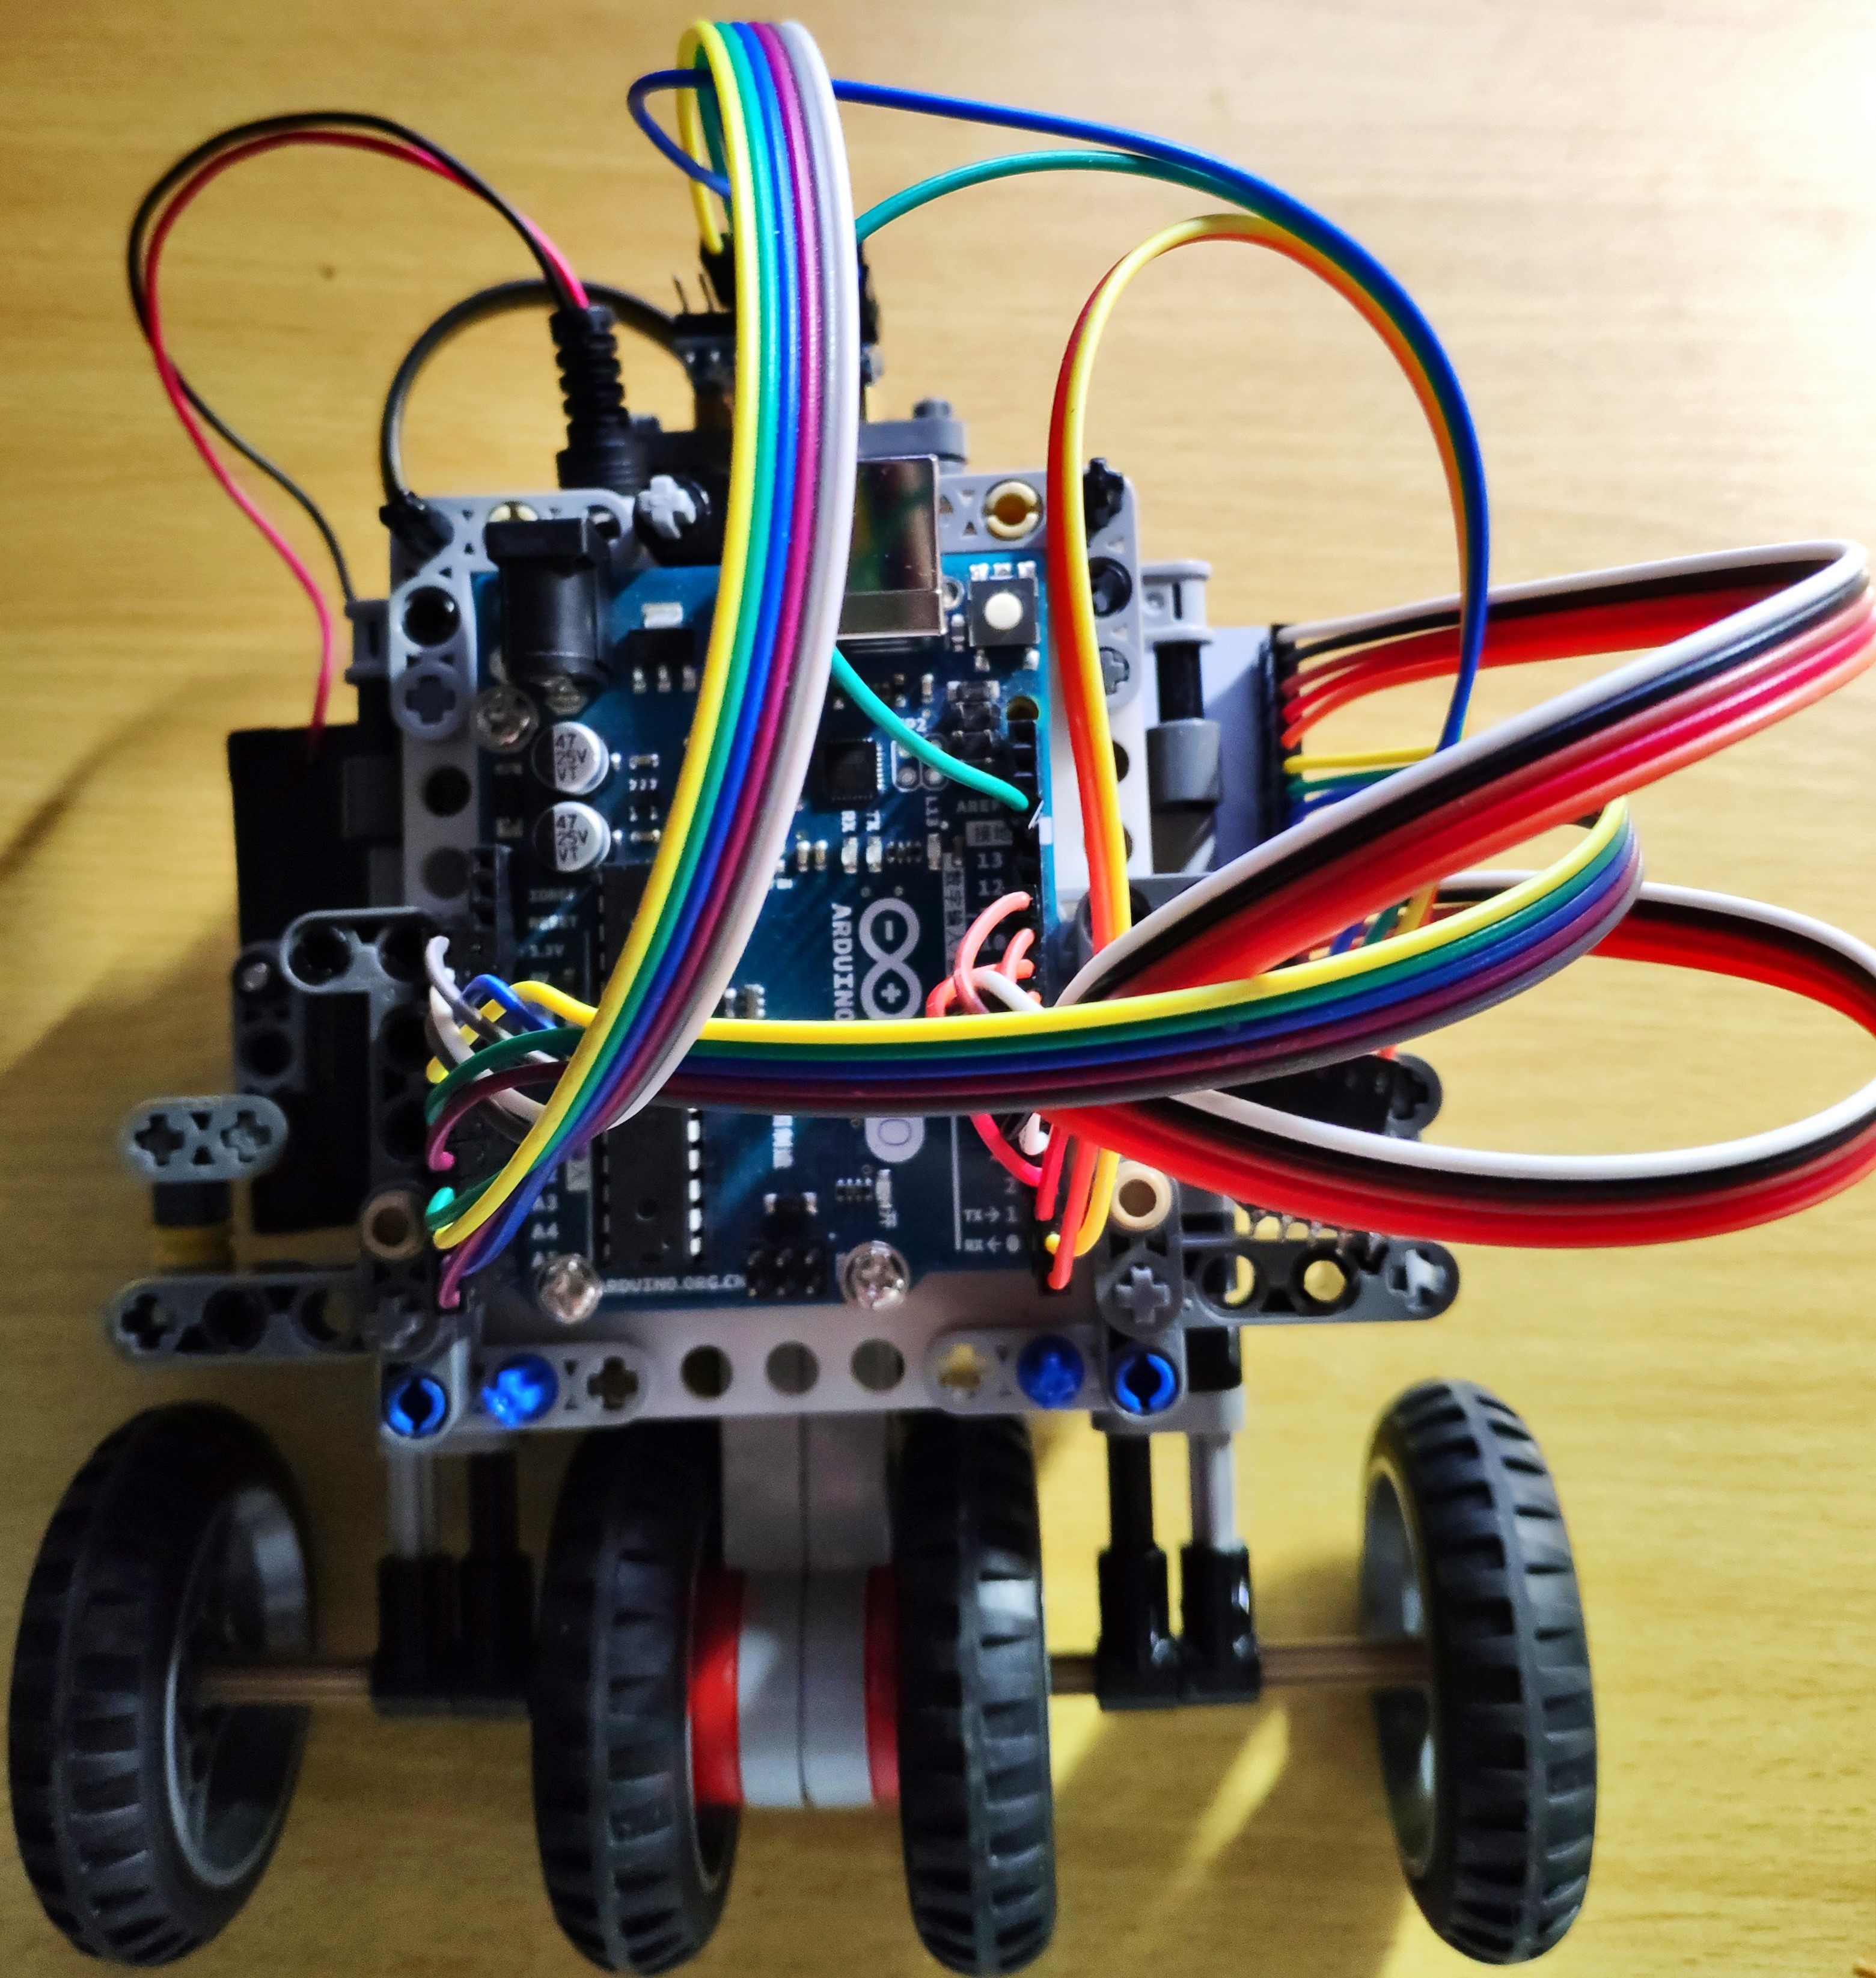
\includegraphics[width=\textwidth]{figure//F2.jpg}
\end{minipage}
\begin{minipage}[t]{0.52\textwidth}
\centering
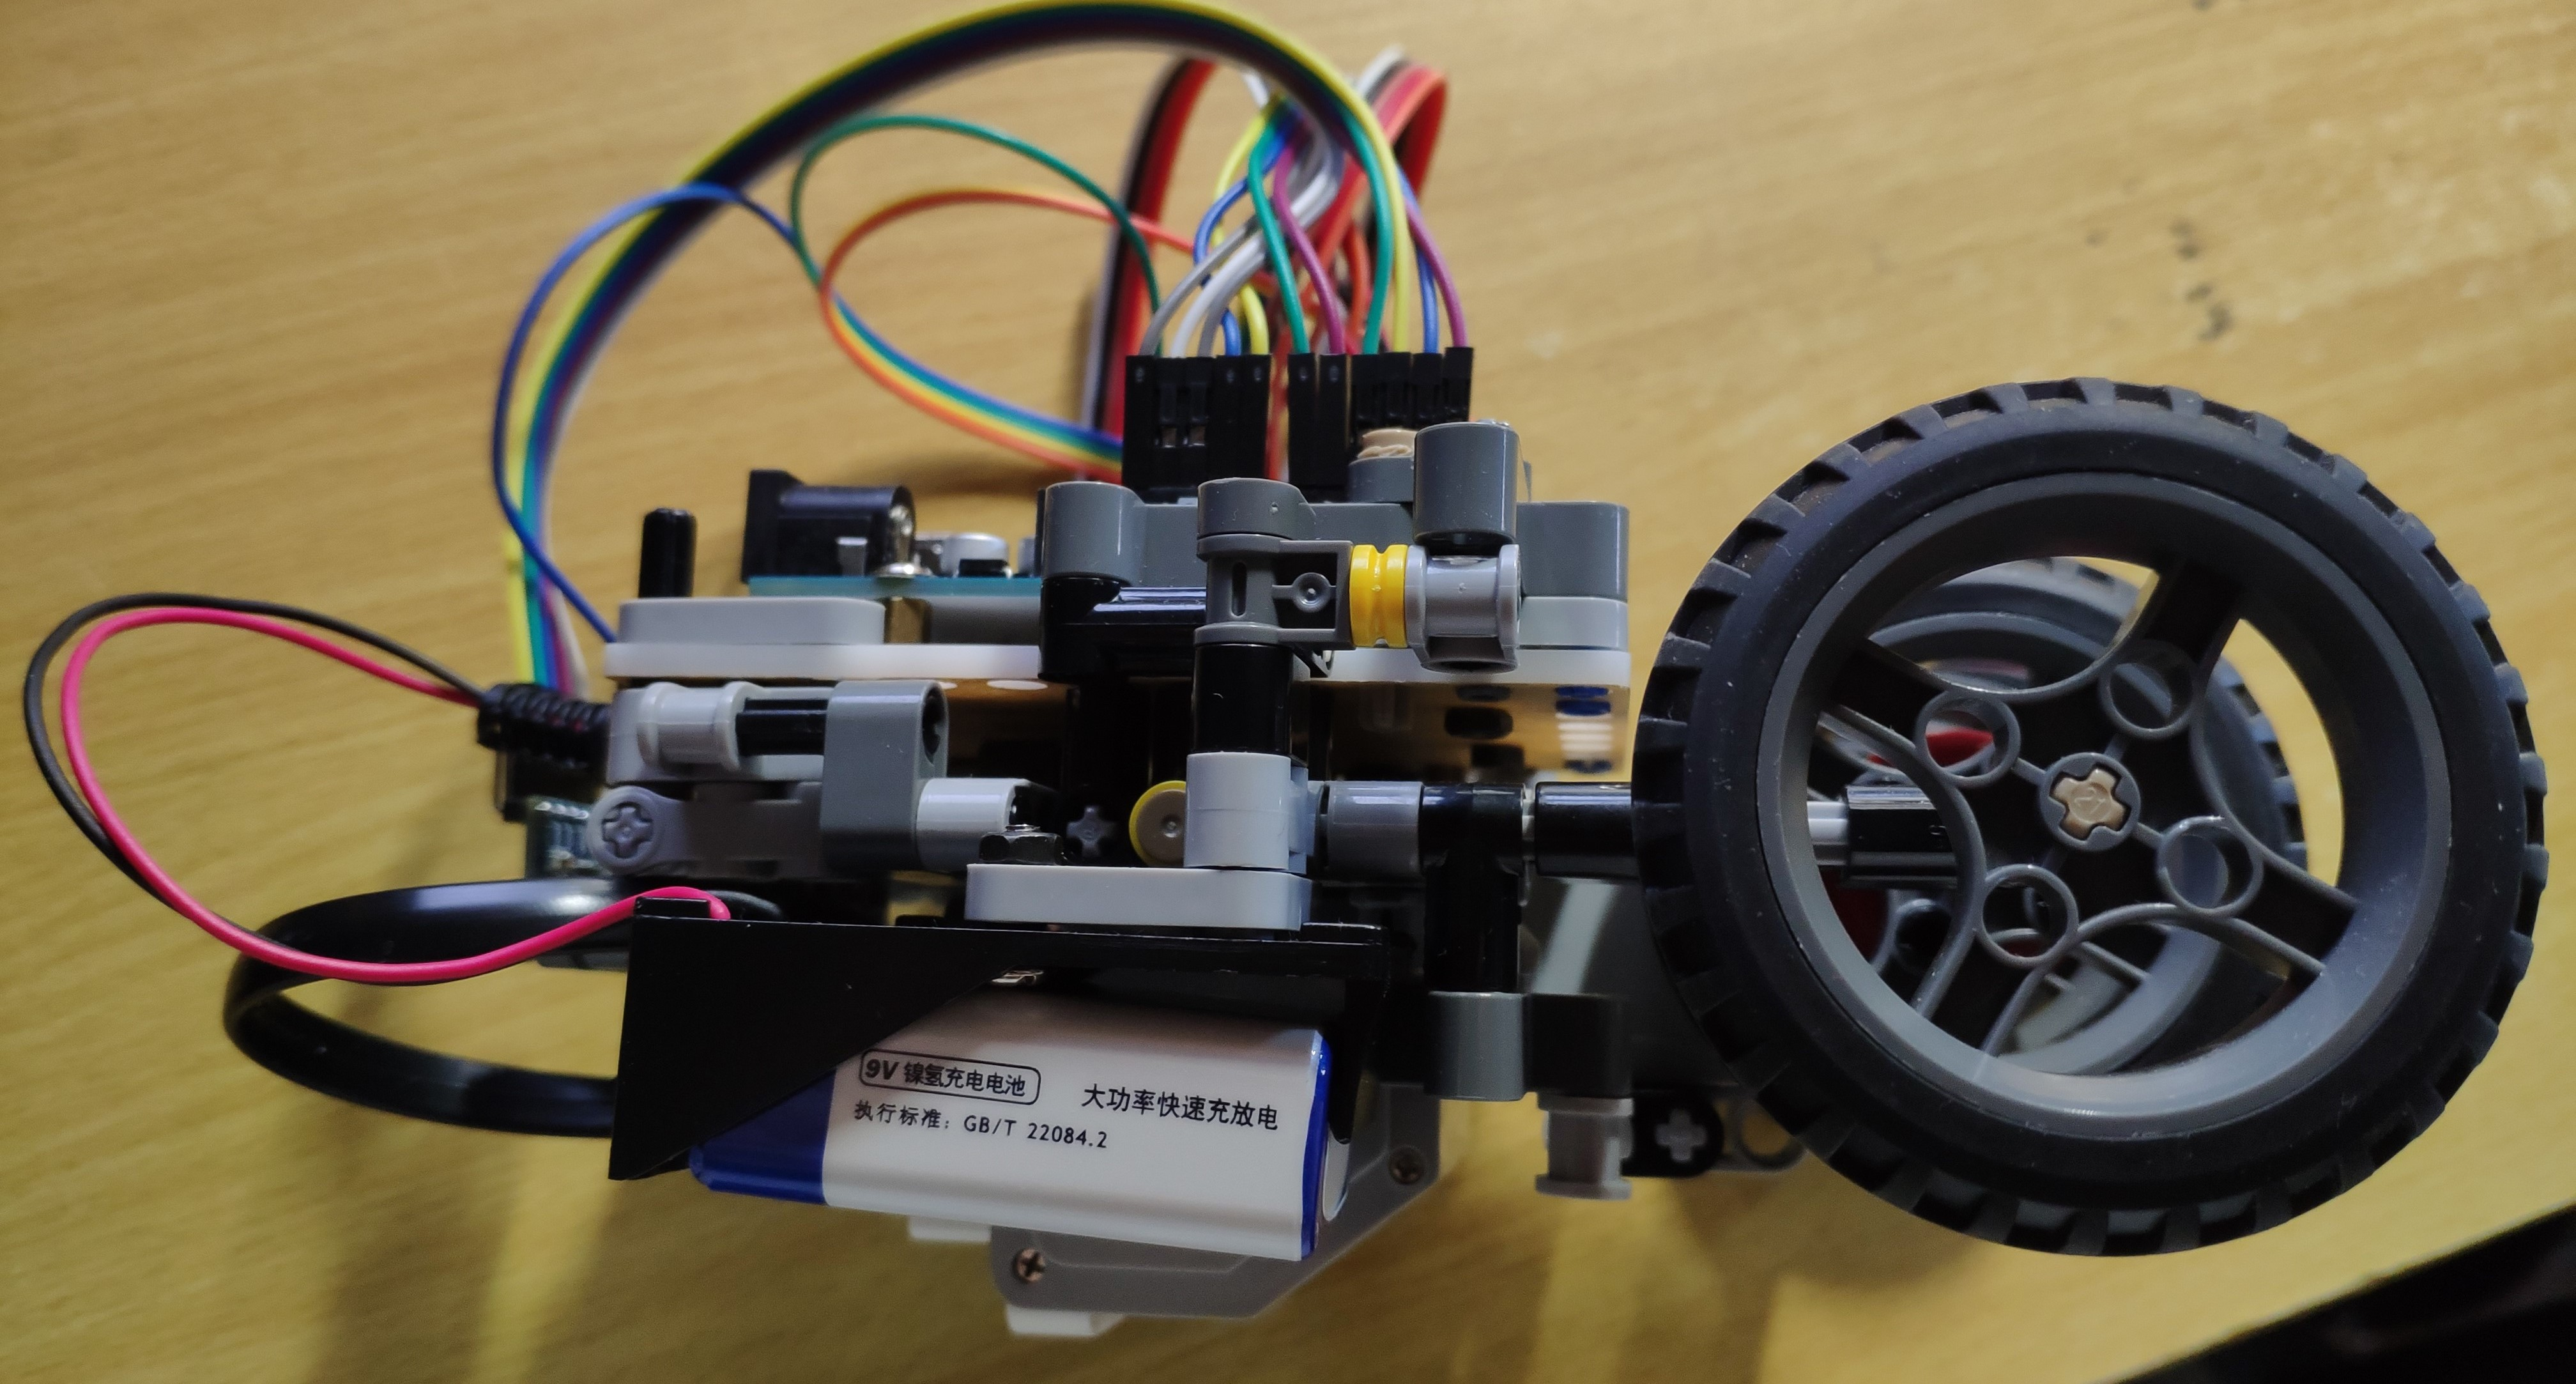
\includegraphics[width=\textwidth]{figure//F3.jpg}
\end{minipage}%
\hfill
\begin{minipage}[t]{0.48\textwidth}
\centering
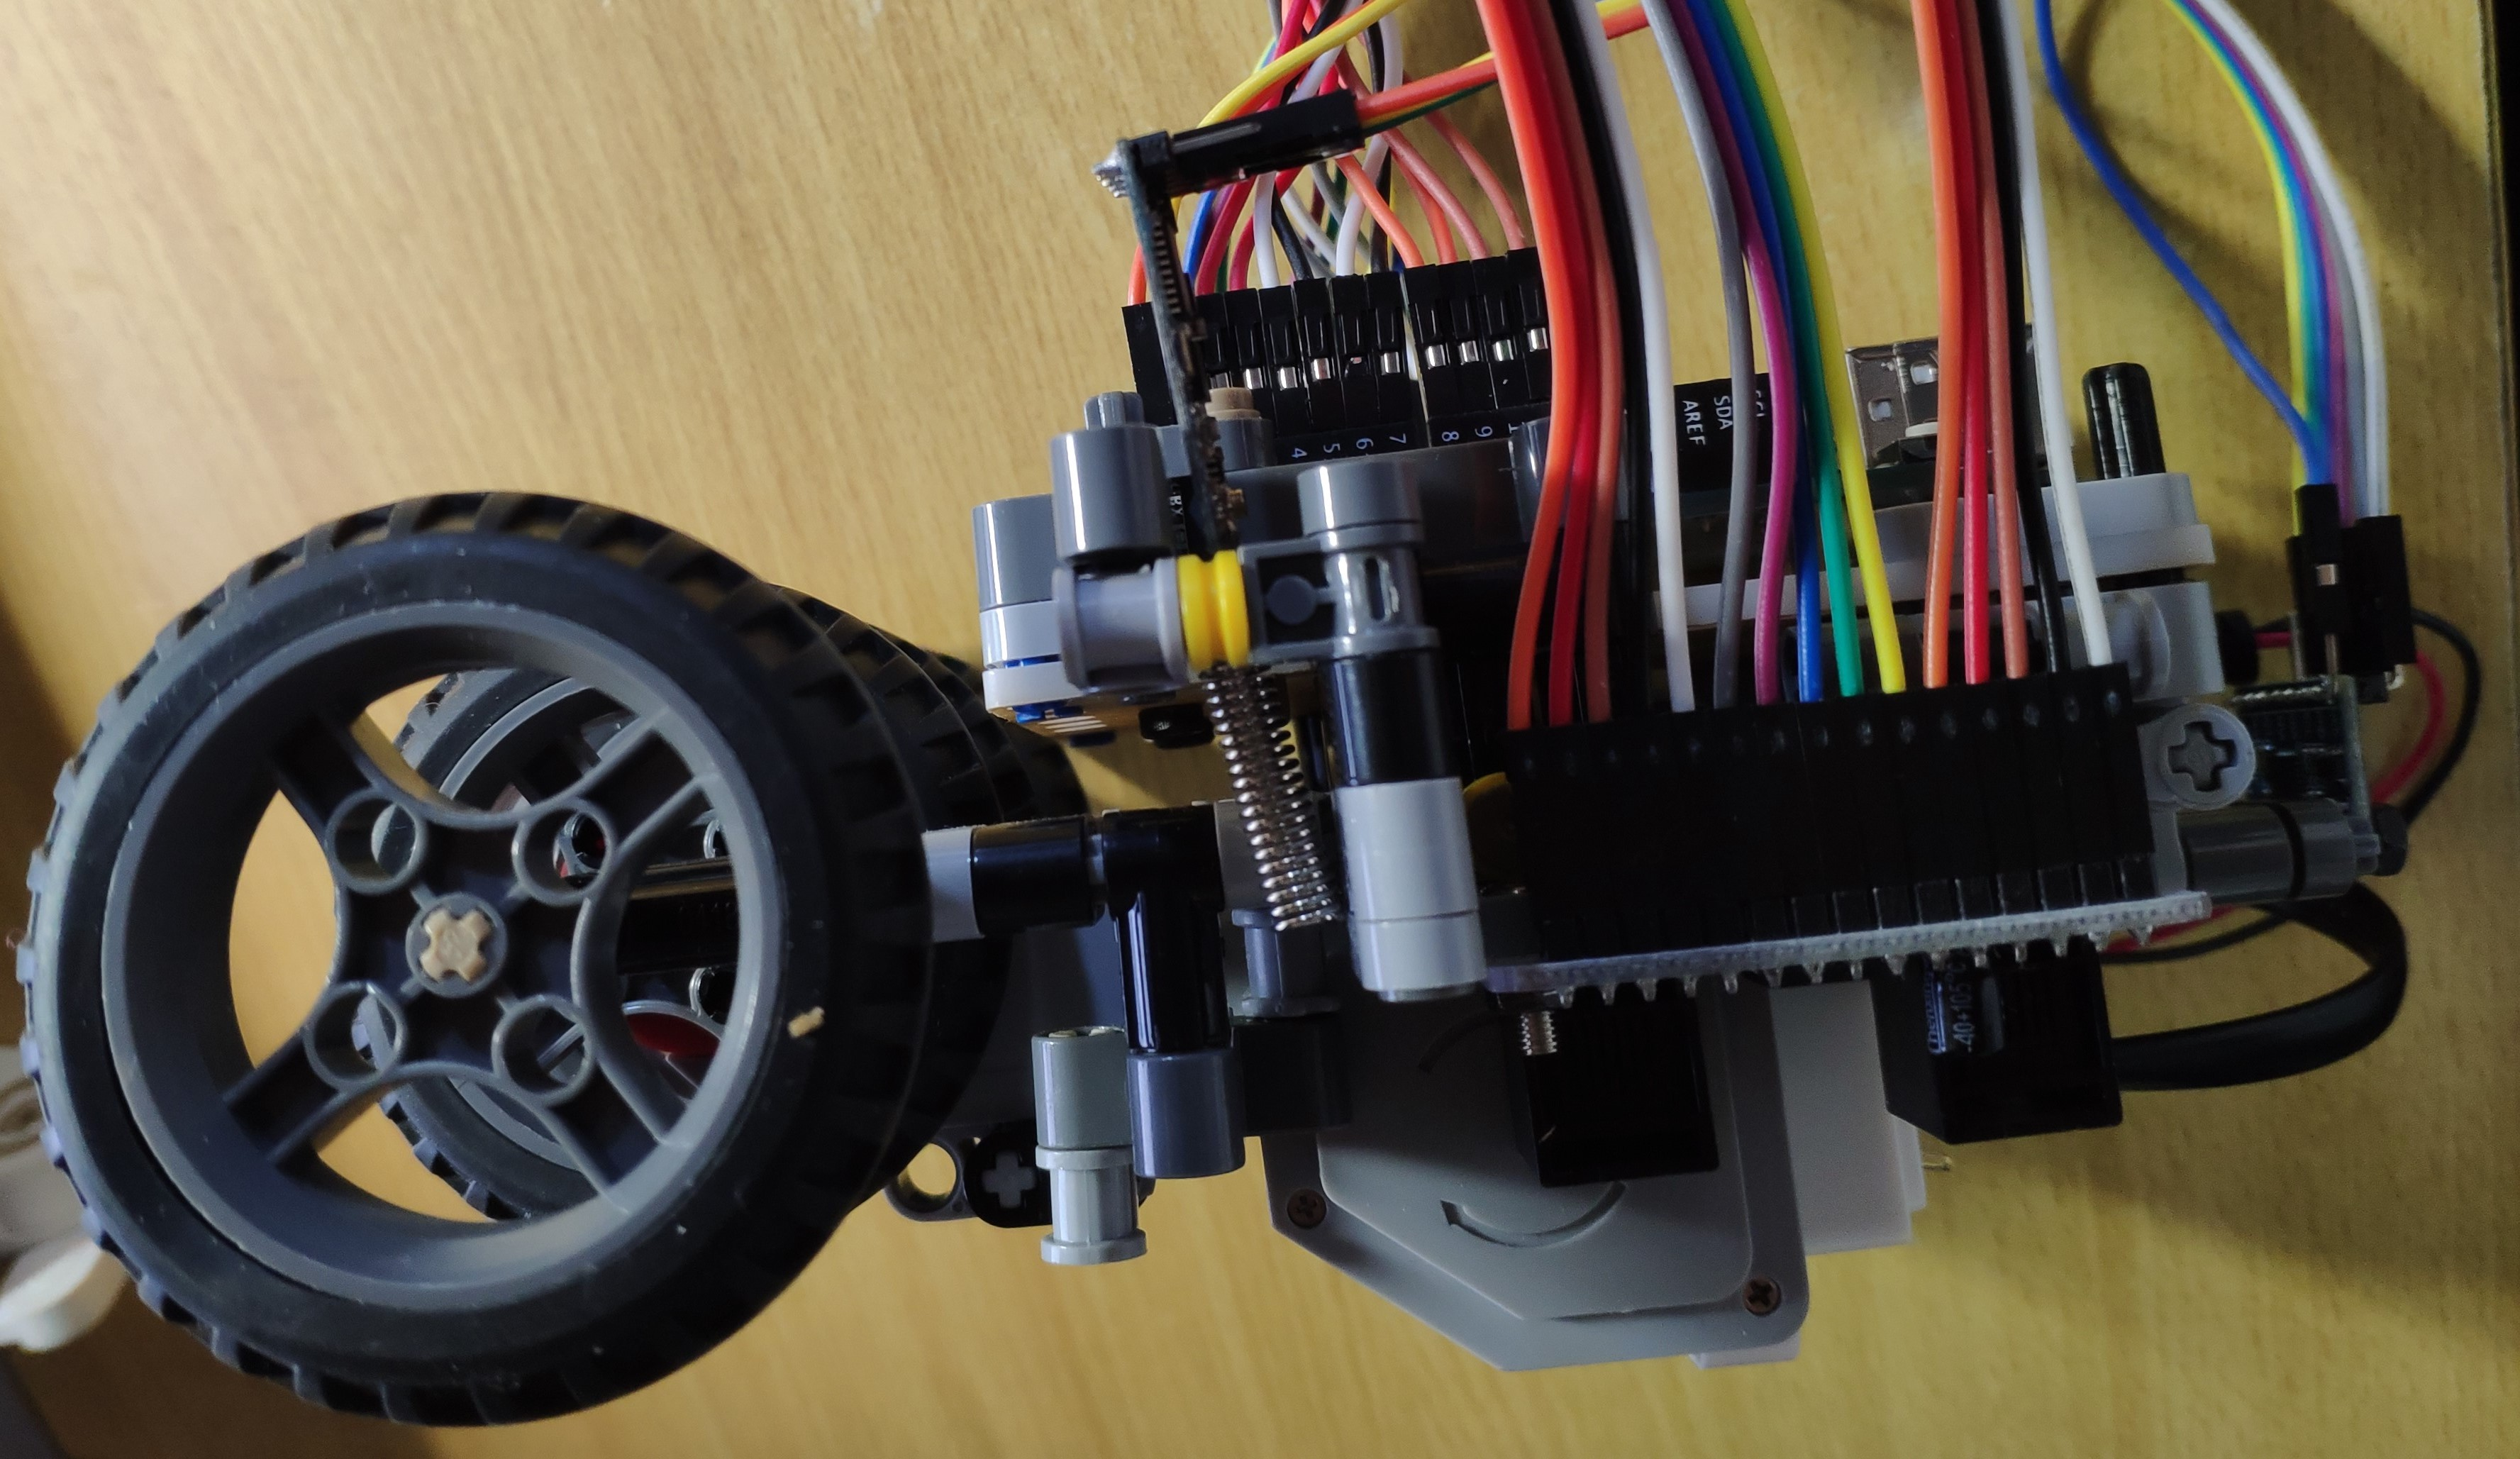
\includegraphics[width=\textwidth]{figure//F4.jpg}
\end{minipage}
\caption{实物图}\label{frame}
\end{figure}
\subsection{程序}
\subsubsection{传感器数据获取}
MPU6050数据获取采用Arduino设备类库中的I2Cdev.h和MPU6050.h类库,调用MPU6050.getMotion6()方法读取三轴角度和加速度数据。

电机编码器数据采用BricktronicsMotorDriver默认类库BricktronicsMotor.h中的BricktronicsMotor.getAngle()方法。
\subsubsection{传感器数据滤波}

传感器数据滤波采用常见的Kalman滤波算法。设在取样时刻t的取样值为$x_{t}$,取样标准差为$\sigma_{t}$,$y_{t}$为滤波值,滤波值标准差为$Q$则在时刻$t$,Kalman滤波算法给出的$x_{t}$和$y_{t}$递推关系式如下:
\begin{equation}
\left\{
\begin{aligned}
P_{t}&=&P_{t-1}(1-K_{t-1})+Q\\
K_{t}&=&\frac{P_{t}}{P_{t}+\sigma_{t}}\\
y_{t}&=&y_{t-1}+K_{t}(x_{t}-y_{t-1})\\
\end{aligned}
\right.
\end{equation}

\newpage
\subsubsection{PID控制}

车轮PWM控制频率采用PID控制算法计算得出。设t时刻角度和角速度传感器经滤波算法测量到的小车倾斜角度值为$\theta(t)$,角速度为$\omega(t)$;编码器得到的车轮角位置为$\theta_{r}(t)$,则PID控制算法输出的车轮PWM控制频率表达式如下:
\begin{equation}
f_{PWM}=k_{p}\theta(t)+k_{i}\int_{0}^{t}\theta(t) dt+k_{d}\omega(t)+k_{sp}\theta_{r}(t)+k_{sd}\frac{d\theta_{r}(t)}{dt}
\end{equation}
实际计算时,将计算出的$\int_{0}^{t}\theta(t) dt$限制在一定范围内,以防止值过大导致其他控制项失效;计算$\frac{d\theta_{r}(t)}{dt}$时,取
$$
d\theta_{r}(t)\approx
\left\{
\begin{aligned}
&\theta_{r}(t)-\theta_{r}(t-1)&-360^\circ 
&&(\theta_{r}(t)-\theta_{r}(t-1)&>=180^\circ)\\
&\theta_{r}(t)-\theta_{r}(t-1)&
&(0^\circ<&\theta_{r}(t)-\theta_{r}(t-1)&<180^\circ)\\
&\theta_{r}(t)-\theta_{r}(t-1)&+360^\circ
&&(\theta_{r}(t)-\theta_{r}(t-1)&<=180^\circ)\\
\end{aligned}
\right.
$$
\subsubsection{PWM控制输出}
电机编码器PWM控制输出采用BricktronicsMotorDriver默认类库BricktronicsMotor.h中的BricktronicsMotor.setFixedDrive()方法。
\section{设计难点}
\begin{enumerate}
	\item 电机减速比过大导致转速不足,进而对PID控制算法的参数调节带来困难。
	\item 边设计边组装的方法无法对小车重心进行精确调节,使传感器角度数据读取和处理的程序中需要增加和重心位置有关的偏置项,进一步增加了参数调节的难度。
	\item 电机编码盘为绝对式编码盘,不利于速度测量。
\end{enumerate}
\section{心得体会}
\begin{itemize}
	\item 了解了单片机设备开发的一般模式
	\item 体会到单片机控制物理系统时,系统设备选择的重要性
	\item 对Kalman滤波算法有了一个初步的理解并能在实际中运用
	\item 在实践中巩固了自动控制原理关于PID控制的知识
\end{itemize}
\end{spacing}

\newpage
\titleformat{\section}{\heiti\Large}{附录}{11pt}{\Large}
\titlespacing{\section}{0pt}{*-4}{*4}
\renewcommand{\thesection}{附录\Alph{section}.} 
\begin{appendices}
\section{程序清单}
\lstset{
	language={[Sharp]C},
	numbers=left,numberstyle=\tiny,
	basicstyle=\small\ttfamily,
	stringstyle=\color{codepurple},
	keywordstyle=\color{blue}\bfseries,
	commentstyle=\color{codegreen},
	frame=shadowbox,
	rulesepcolor=\color{codegray}
}
\begin{lstlisting}
#include "Wire.h"
#include "I2Cdev.h"
#include "MPU6050.h"
#include <BricktronicsMotor.h>

MPU6050 accelgyro;
int16_t ax, ay, az, gx, gy, gz;             //加速度计陀螺仪原始数据
float aay = 0, agy = 0; //角度变量
long ayo = 0;             //加速度计偏移量
long gyo = 0;             //陀螺仪偏移量
void mpu_init()//传感器初始化
{
Wire.begin();
accelgyro.initialize();                 //传感器初始化
unsigned short times = 200;             //采样次数
for (int i = 0; i < times; i++)
{
accelgyro.getMotion6(&ax, &ay, &az, &gx, &gy, &gz); //读取六轴原始数值
ayo += ay;      //采样和
gyo += gy;
}
ayo /= times;//计算加速度计偏移
gyo /= times;//计算陀螺仪偏移
}

unsigned long now, lastTime = 0;
float dt;                                   //微分时间
void time_get()//计算时间
{
now = millis();             //当前时间(ms)
dt = (now - lastTime) / 1000.0;           //微分时间(s)
lastTime = now;                           //上一次采样时间(ms)
}


float pi = 3.1415926;
float AcceRatio = 16384.0;                  //加速度计比例系数
float GyroRatio = 131.0;                    //陀螺仪比例系数
uint8_t n_sample = 8;                       //加速度计滤波算法采样个数
float aays[8] = {0};         //x,y轴采样队列
long aay_sum;                     //x,y轴采样和
float gyroy;
void mpu_get()//获取mpu数据
{
accelgyro.getMotion6(&ax, &ay, &az, &gx, &gy, &gz); //读取六轴原始数值
float accx = ax / AcceRatio;              //x轴加速度
float accy = ay / AcceRatio;              //y轴加速度
float accz = az / AcceRatio;              //z轴加速度
aay = atan(accx / accz) * 180 / pi;       //x轴对于z轴的夹角
aay_sum = 0;                              // 对于加速度计原始数据的滑动加权滤波算法
for (int i = 1; i < n_sample; i++)
{
aays[i - 1] = aays[i];
aay_sum += aays[i] * i;
}
aays[n_sample - 1] = aay;                      //此处应用实验法取得合适的系数
aay_sum += aay * n_sample;                     //本例系数为9/7
aay = (aay_sum / (11 * n_sample / 2.0)) * 9 / 7.0; //角度调幅至0-90°
gyroy = - (gy - gyo) / GyroRatio * dt; //y轴角速度
agy += gyroy;                             //y轴角速度积分
}


float a_y[10] = {0}, g_y[10] = {0}; //加速度计协方差计算队列
float Py = 1, Ry, Ky, Sy, Vy, Qy = 0.01;         //y轴卡尔曼变量
void mpu_kalman()//计算Kalman滤波
{
Sy = 0; Ry = 0;
for (int i = 1; i < 10; i++)
{ //测量值平均值运算
a_y[i - 1] = a_y[i];                    //即加速度平均值
Sy += a_y[i];
}
a_y[9] = aay;
Sy += aay;
Sy /= 10;                                 //y轴加速度平均值

for (int i = 0; i < 10; i++)
{
Ry += sq(a_y[i] - Sy);
}
Ry = Ry / 9;
//求加速度方差
Py = Py + Qy;                         // 0.0025在下面有说明...
Ky = Py / (Py + Ry);                      //计算卡尔曼增益
agy = agy + Ky * (aay - agy);             //陀螺仪角度与加速度计速度叠加
Py = (1 - Ky) * Py;                       //更新p值
}

BricktronicsMotor m(4, 5, 10, 2, 8);
int16_t m_position_last;//上一循环的电机位置
void motor_init()//电机初始化
{
m.begin();
m_position_last = m.getAngle(); //获取电机初始角度
}

int16_t m_position;//电机位置
int16_t motor_difs[10] = {0}; //电机位置差
int16_t motor_dif = 0;
float m_speed = 0;
float motor_position = 0;
void motor_get()
{
m_speed = 0;
for (int i = 1; i < 10; i++)
{ //测量值平均值运算
motor_difs[i - 1] = motor_difs[i];                    //即加速度平均值
m_speed += motor_difs[i];
}
m_position = m.getAngle();
motor_dif = m_position - m_position_last;
if (motor_dif >= 180)motor_dif = motor_dif - 360;
else if (motor_dif <= -180)motor_dif = 360 + motor_dif;
motor_difs[9] = motor_dif;
m_speed += motor_dif;
m_speed /= dt * 10;
m_position_last = m_position;
motor_position += motor_dif; //计算马达位置
}

void motor_position_get()
{
if (motor_position > 180) motor_position = 180;
if (motor_position < -180) motor_position = -180;
}

float motor_speed = 0;
float m_s[10] = {0}; //电机速度协方差计算队列
float Pm = 1, Rm, Km, Sm, Vm, Qm = 100;         //卡尔曼变量
void motor_kalman()
{
Sm = 0; Rm = 0;
for (int i = 1; i < 10; i++)
{ //测量值平均值运算
m_s[i - 1] = m_s[i];
Sm += m_s[i];
}
m_s[9] = m_speed;
Sm += m_speed;
Sm /= 10;
//求电机速度平均值

for (int i = 0; i < 10; i++)
{
Rm += sq(m_s[i] - Sm);
}
Rm = Rm / 9;
//求电机速度测量方差

Pm = Pm + Qm;
Km = Pm / (Pm + Rm);
motor_speed = motor_speed + Km * (m_speed - motor_speed);
Pm = (1 - Km) * Pm;
}

void setup()
{
Serial.begin(115200);
mpu_init();
motor_init();
}

int32_t PWM;
int16_t pwm;
void pwm_get()
{
if (PWM >= 255)pwm = 255;
else if (PWM <= -255)pwm = -255;
else pwm = PWM;
pwm = -pwm;
}

float error_I = 0;
float error_D = 0;
float error = 0;
float Imax=1500;
void Ierror()
{
error_I += error;
if (error_I > Imax)error_I = Imax;
if (error_I < -Imax)error_I = -Imax;
}

float kp = 210;
float ki = 0;
float kd = 2300;
float ksp = 0;
float ksd = 0;
#define CMD_IMG 3
uint8_t cmdf[2] = {CMD_IMG, ~CMD_IMG};
uint8_t cmdr[2] = {~CMD_IMG, CMD_IMG};
float send_out[3];
void loop()
{
time_get();
mpu_get();
mpu_kalman();
motor_get();
motor_position_get();
motor_kalman();
error = agy - 0.236;
Ierror();
error_D = gyroy;

PWM = error * kp + error_I * ki + error_D * kd + motor_position * ksp + motor_speed * ksd;
pwm_get();
m.setFixedDrive(pwm);

send_out[0] = error;
send_out[1] = (float)pwm;
send_out[2] = error_I;
Serial.write(cmdf[0]);
Serial.write(cmdf[1]);
Serial.write((char *)send_out, 3 * sizeof(float));
Serial.write(cmdr[0]);
Serial.write(cmdr[1]);

}
\end{lstlisting}
\end{appendices}
\end{document}